\documentclass[journal]{IEEEtran}
\usepackage{amsmath,amssymb}
\usepackage{algorithm,algorithmic}
\usepackage{booktabs}
\usepackage{subfigure}
\usepackage{graphicx}
\usepackage{cite}
\usepackage{url}
\usepackage{xcolor}

\newcommand{\npie}{\textsc{NPIE}}
\newcommand{\tx}{\boldsymbol{\theta}_{\mathrm{Tx}}}
\newcommand{\rx}{\boldsymbol{\theta}_{\mathrm{Rx}}}
\newcommand{\rxp}{\boldsymbol{\theta}_{\mathrm{Rx},p}}
\newcommand{\xmark}{$\times$}

\begin{document}

\title{Neural-Physical Interpretable RF Fingerprint Identification:\\Disentangling Transmitter Impairments from Receiver and Time Shifts}

\author{
Anonymous Authors\\
Manuscript submitted for peer review
}

\maketitle

\begin{abstract}
RF fingerprint identification (RFFI) must generalize across two deployment shifts that black-box state-of-the-art methods fail to survive jointly: \emph{cross-receiver} hardware mismatch and \emph{cross-time} temperature/aging drift. Existing leaders on the WiSig ManySig benchmark (e.g.\ WaveMLP, 93.13\%) are IQ/STFT/wavelet frontends on ResNet/MLP backbones that are opaque and provide no interpretable fingerprint. We propose \npie\ (Neural-Physical Interpretable RFFI), a resolution-preserving complex frontend coupled with an explicit physical-impairment estimator $\tx$ that is made invariant to receiver and time shifts through supervised contrastive and gradient-reversal training, plus a train-time random phase-augmentation that forces rotation-invariant features. On the WiSig ManySig cross-receiver$\times$cross-day (CRD) protocol, \npie\ reaches \textbf{96.64\%}, beating the fair-budget WaveMLP@1000 baseline (95.04\%) by \textbf{+1.60\,pp} and exceeding its entire 3-seed range (92.53--95.00\%). Under maximum temporal drift (hardday) it gains \textbf{+5.60\,pp} (97.93\% vs 92.33\%), and under leave-one-receiver-out it holds \textbf{97.58\%}. \npie\ further exceeds the only joint receiver+time SOTA (DRIFT) by \textbf{$>$17\,pp} on both axes. Crucially, the learned $\tx$ yields a transmitter fingerprint whose within-device clustering is \textbf{19$\times$ tighter} than the no-disentanglement baseline and reaches \textbf{63.5\%} under a nearest-centroid probe (random 16.7\%)---interpretability that no black-box competitor offers. To our knowledge \npie\ is the first physically-interpretable RFFI method that also surpasses black-box SOTA on accuracy, stability, and dual-offset robustness.
\end{abstract}

\begin{IEEEkeywords}
RF fingerprint identification, specific emitter identification, physical-layer security, interpretable deep learning, cyclostationarity, domain adaptation, hardware impairment.
\end{IEEEkeywords}

% =====================================================================
\section{Introduction}
\label{sec:intro}
% =====================================================================
\IEEEPARstart{R}{F} fingerprint identification (RFFI), also called specific emitter identification (SEI), exploits the minute, hard-to-forge imperfections of a transmitter's radio-frequency frontend---power-amplifier (PA) nonlinearity, oscillator phase noise, I/Q imbalance, and carrier-frequency offset---as a physically rooted device identity at the physical layer. Because these impairments originate in analog hardware that is \emph{manufactured}, not \emph{configured}, they are difficult to clone or spoof, which makes RFFI attractive for spectrum-access authentication, rogue-drone detection, device admission control in the Internet of Things, and maritime/satellite emitter tagging. In the laboratory---one receiver, one day of capture, a closed set of devices---closed-set accuracy routinely exceeds 99\%. In the field, that number does not survive contact with reality, because the \emph{capture condition} changes. Two shifts dominate the decay.

\textbf{Cross-receiver shift.} The same transmitter captured by a different software-defined radio passes through different I/Q offset, local-oscillator drift, gain/phase response, anti-alias filtering, and automatic gain control. The fingerprint the model learned is now convolved with hardware it has never seen. Shen~et~al.~\cite{shen2024} quantify the damage and the remedy: a single-receiver model must be augmented by +20\% multi-receiver collaborative inference, or +40\% fine-tuning, merely to recover its original accuracy when the receiver changes. The implication is uncomfortable---a large fraction of what an opaque model learns is not the transmitter at all, but the receiver it happened to be captured with.

\textbf{Cross-time shift.} Temperature drift and crystal aging slowly morph the fingerprint over hours, days, and months. Longitudinal studies report that a 96\% laboratory model decays to $\sim$50\% across days and to $\sim$40\% across deployment environments~\cite{quadar2024}, and a simple power cycle---the afterglow effect of a warm versus cold oscillator---can halve accuracy~\cite{alhazbi}. The fingerprint is not a static signature; it is a slowly drifting trajectory, and a model trained on one point of that trajectory silently degrades on all others.

Either shift alone is survivable with enough data augmentation or adaptation. The two \emph{jointly}---which is the real deployment condition: a different receiver, on a different day---are not. \textbf{Threat and deployment model.} Throughout, we assume a closed set of legitimately enrolled transmitters and an operator who controls the training receivers and schedule; the adversary is the environment itself (unplanned receivers, unplanned time), not an active spoofer. This is the setting of the ManySig benchmark and of the deployment scenarios motivating it---drone fleets, IoT admission control, spectrum monitoring---where the practical question is not ``can the model recognize a device it was trained on, in the lab it was trained in'' but ``how much accuracy survives when neither condition holds.'' Spoofing and adversarial-IQ attacks are orthogonal and out of scope.

The current ManySig leader, WaveMLP~\cite{wavemlp}, reports 93.13\% on the cross-receiver$\times$cross-day (CRD) protocol, while the \emph{same family} of methods reaches 99.78\% when \emph{only the day varies}~\cite{belfast2026}. The joint shift costs roughly 7\,pp over the time-only shift; that gap is the price of receiver variation entangled with drift, and closing it is the accuracy goal of this paper.

The two shifts are also \emph{asymmetric} in a way that matters for design. Cross-receiver distortion is dominated by linear, quasi-static filtering: it changes the observation but not the emitter, and it can in principle be measured, calibrated, or adversarially removed. Cross-time drift is slower but subtler: it acts \emph{inside} the transmitter itself (warm-up, aging, thermal expansion), so the fingerprint genuinely moves, and part of that movement is indistinguishable from an identity change at single-capture resolution. A method that treats both shifts as one generic ``domain gap'' must find a single representation that is simultaneously invariant to an external linear operator and to a slow internal parameter walk. That is a strong requirement to impose blindly---and a central reason we prefer to impose it on an explicit physical quantity whose invariance can be checked.

The deeper problem is that the current leaders are \emph{black boxes}. WaveMLP~\cite{wavemlp}, Feng~et~al.~\cite{feng2025} (92.52\%), and Bulugu~\cite{bulugu2025} (93.4\% after fine-tuning) learn IQ/STFT/wavelet features on ResNet/MLP backbones and report an accuracy number, but offer no evidence of \emph{what} the model locks onto, no reason to trust it under drift, and no physical interpretation. This is not merely an aesthetic deficiency. Interpretability matters operationally for at least four reasons. First, in forensics and legal intercept, an identification that cannot be explained is difficult to admit as evidence. Second, for certification and regulatory acceptance, an operator must be able to inspect \emph{which} hardware property identifies the emitter. Third, a model whose features are entangled with capture condition fails silently under drift; an explicit, inspectable fingerprint makes the failure diagnosable. Fourth, knowing what the model locks onto is the only reliable predictor of robustness under distribution shift---a model that locks onto the receiver will not survive a receiver change, no matter how high its validation accuracy. WaveMLP, Feng, Bulugu, and the joint-offset DRIFT method all use signal-energy or disentangled latent features; none use cyclostationary structure, and none expose a hardware-impairment estimate.

We take a different stance: rather than learn ``yet another black-box feature,'' we \emph{explicitly estimate} the transmitter's hardware-impairment parameters $\tx$ and \emph{constructively make them invariant} to receiver and time distortion. The payoff is twofold. First, $\tx$ is a genuine, inspectable fingerprint: we can measure whether same-transmitter estimates cluster tightly across all receivers and days, and whether they carry any residual capture-condition information, and report those measurements as hard evidence. Second, invariance to drift becomes a built-in property of the representation rather than a hoped-for emergent one---which is exactly what survives the joint receiver$\times$time shift.

\textbf{Contributions.} This paper makes the following contributions:
\begin{enumerate}
\item We propose \npie, a resolution-preserving \emph{complex} frontend followed by an explicit physical-impairment estimator $\tx$ and a supervised-contrastive + gradient-reversal (GRL) invariance head that disentangles transmitter identity from receiver/time conditions.
\item We introduce a train-time \emph{random phase-augmentation} ($e^{j\phi}$, $\phi\sim\mathcal{U}(0,2\pi)$) that forces rotation-invariant features; it is the single largest accuracy lever (+1.78\,pp on CRD) and the mechanism behind cross-time robustness.
\item On WiSig ManySig CRD, \npie\ reaches 96.64\%, exceeding the fair-budget WaveMLP@1000 by +1.60\,pp and exceeding \emph{every} seed of that baseline (whose 3-seed mean is only $93.82\pm1.01\%$). It further gains +5.60\,pp on hardday and holds 97.58\% under leave-one-receiver-out.
\item We close the \emph{dual-offset} claim with real data: \npie\ beats the only joint receiver+time SOTA (DRIFT, 75.62\%/79.27\%) by $>$17\,pp on both axes, and the learned $\tx$ exhibits 19$\times$ tighter same-transmitter clustering with a 63.5\% centroid-probe fingerprint---interpretability absent from all black-box baselines.
\end{enumerate}

The remainder of the paper is organized as follows. Section~\ref{sec:related} surveys related work. Section~\ref{sec:model} formalizes the signal model and the two shifts. Section~\ref{sec:method} presents \npie. Section~\ref{sec:exp} reports experiments on WiSig ManySig and UAV-Sigmf, including ablations and the dual-offset closure. Section~\ref{sec:interp} analyzes the interpretability of $\tx$, Section~\ref{sec:discussion} discusses limitations, and Section~\ref{sec:conclusion} concludes.

% =====================================================================
\section{Related Work}
\label{sec:related}
% =====================================================================
\subsection{Black-box cross-receiver RFFI}
WaveMLP~\cite{wavemlp} learns a complex wavelet (LCWT) on an MLP backbone and reports 93.13\% on ManySig CRD, the largest public cross-receiver$\times$cross-day benchmark. Feng~et~al.~\cite{feng2025} pair a ResNet18 frontend with dynamic MMD/LMMD distribution alignment and reach 92.52\%; the alignment is applied to latent features but the frontend itself remains an opaque CNN. Bulugu~\cite{bulugu2025} uses SE-attention within a multi-source domain-adversarial network and moves from 83.3\% to 93.4\% only after target-domain fine-tuning, i.e.\ the invariance is bought with labeled or semi-labeled target access. Shen~et~al.~\cite{shen2024} attack the cross-receiver problem directly with adversarial receiver-agnostic features plus collaborative inference, and quantify the +20\%/+40\% recovery overhead noted above. All of these are feature learners with no invariance \emph{guarantee}, no interpretable output, and no mechanism that separates the transmitter's contribution from the receiver's. \npie\ differs in kind, not degree: it estimates an explicit physical quantity and constructs the invariance.

\textbf{What the leaders actually learn.} A recurring finding across these studies is that a substantial share of the learned representation is capture-condition-specific: models fine-tuned to a new receiver recover tens of points~\cite{shen2024}, alignment losses must close large distributional distances~\cite{feng2025}, and receiver-diverse augmentation is consistently the strongest regularizer. None of these papers reports a measurement that isolates how much of the feature is transmitter versus receiver; the question is not asked. Our experimental design makes it answerable by construction---the physical branch is architecturally discouraged from absorbing receiver identity (it is regressed toward a transmitter-side quantity, decorrelated from a receiver estimate, and adversarially stripped of receiver/day information), and the disentanglement ratio measures whatever residue remains.

\subsection{Cross-time drift}
Deployment-decay studies quantify the cross-day collapse (96\%$\to$50\%)~\cite{quadar2024} and the power-cycle halving~\cite{alhazbi}. Domain-adversarial training~\cite{ganin2016} is known to neutralize time shift by mapping day-1 and day-100 samples of one device to the same latent region, and it underlies several of the cross-receiver methods above. Recent cross-day unsupervised domain adaptation on ManySig reaches 99.78\% \emph{when only the day varies}~\cite{belfast2026}---demonstrating that time shift, taken alone, is essentially solved by modern UDA. The difficulty lies in the \emph{joint} receiver+time shift, which is the CRD setting (93.13\%): the two nuisances are correlated through the capture schedule, and a model that discards one often discards transmitter-relevant structure with it.

Mechanistically, cross-time drift arises from thermal cycling of the oscillator and PA bias network, slow crystal aging, and recalibration events, each with a different time constant---hours for warm-up, days to weeks for thermal-seasonal effects, months for aging. A 4-day collection samples the first two regimes but not the third; this is a genuine limitation of every ManySig-based claim, including ours, and the reason we describe the hardday result as evidence on \emph{short-horizon} drift rather than a certificate of year-scale invariance.

\subsection{Physical / interpretable RFFI}
The nearest neighbors are model-driven impairment estimators, physics-informed networks, and feature-disentanglement approaches. Yang~et~al.~\cite{yang2026} estimate soft latent impairment variables in a model-driven architecture, but provide no clustering proof that the estimate is capture-condition-free and no constructive invariance mechanism. PINN- and CFO-guided methods inject physical priors into the frontend yet still report a single accuracy number without inspectable fingerprints. DRIFT~\cite{drift} (Pan/Xu/Cheng, arXiv:2510.09405) is the only published method targeting \emph{both} offsets jointly, via feature disentanglement into transmitter and nuisance subspaces; it reports 75.62\% cross-receiver and 79.27\% cross-day and gives no interpretable fingerprint. \npie\ differs on three combined points absent elsewhere: an \emph{explicit} $\tx$ with a regression objective, supervised-contrastive + GRL \emph{constructive} invariance, and \emph{hard evidence} of fingerprint quality (clustering compactness and a centroid probe).

\subsection{Cyclostationary heritage}
Second-order cyclostationarity---the statistical periodicity of modulated signals at cycle frequencies tied to the carrier and symbol rate---has been a mainstay of signal-level emitter analysis since Gardner's foundational work~\cite{gardner1988}. Classical SEI used hand-crafted cyclic spectral features; modern deep RFFI largely abandoned them in favor of learned IQ/STFT features. \npie\ occupies the middle ground: its complex, resolution-preserving frontend is designed to \emph{preserve} the second-order periodic structure that real-valued downsampling convolutions destroy (Sec.~\ref{sec:complex}), while the physical branch estimates the impairments that generate the cyclic signature in the first place.

\subsection{Positioning}
Table~\ref{tab:related} summarizes the positioning. No prior method combines a joint receiver+time evaluation, an interpretable output, and a constructive invariance mechanism; each competitor contributes at most one of the three.

\begin{table}[t]
\centering
\footnotesize
\caption{Positioning against the most relevant prior work. ``Joint'' = evaluates cross-receiver and cross-time shift simultaneously. ``Interpretable'' = exposes a \emph{measured} capture-condition-free fingerprint.}
\label{tab:related}
\begin{tabular}{@{}lccc@{}}
\toprule
Method & Joint Rx+Time & Interpretable & Invariance \\
\midrule
WaveMLP~\cite{wavemlp} & \checkmark & \xmark & none \\
Feng~\cite{feng2025} & \xmark & \xmark & MMD/LMMD \\
Bulugu~\cite{bulugu2025} & \xmark & \xmark & multi-src DANN \\
Shen~\cite{shen2024} & \xmark & \xmark & adv.+collab. \\
DRIFT~\cite{drift} & \checkmark & \xmark & disentangle \\
Yang~\cite{yang2026} & \xmark & partial & joint training \\
\textbf{\npie\ (ours)} & \checkmark & \checkmark & SupCon+GRL+phase \\
\bottomrule
\end{tabular}
\end{table}

The table clarifies two frequently conflated claims. First, ``interpretable'' is used here in a strict sense: the method must expose a quantity that is \emph{measured} to be capture-condition-free, not merely a latent named ``transmitter.'' Second, ``joint'' is a property of the evaluation, not the architecture: a method tested only cross-receiver makes no statement about drift, regardless of its internals. \npie\ is the only entry satisfying both, which is what allows the dual-offset claim of Sec.~\ref{sec:closure} to be closed with data rather than by argument.

% =====================================================================
\section{System Model and Preliminaries}
\label{sec:model}
% =====================================================================
\subsection{Signal and impairment model}
Let $x[n]\in\mathbb{C}$ be the complex baseband IQ of one transmitter, captured by receiver $r$ on day $d$. The received signal decomposes as
\begin{equation}
x[n] = h_{r,d}\big(\,s[n;\tx]\,\big) + w[n],
\label{eq:signal}
\end{equation}
where $s[n;\tx]$ is the transmitter's emission parameterized by its hardware impairments $\tx$, $h_{r,d}(\cdot)$ is the receiver/time transfer function, and $w[n]$ is noise. The emission is shaped by three dominant impairment families, each device-specific because of component tolerances.

\textbf{PA nonlinearity.} With the widely used Saleh model~\cite{saleh1981}, an input envelope $r[n]=|s_{\mathrm{lin}}[n]|$ is distorted by
\begin{equation}
A(r) = \frac{g_a r}{1+\beta_a r^2}, \qquad
\Phi(r) = \frac{g_\phi r^2}{1+\beta_\phi r^2},
\label{eq:saleh}
\end{equation}
producing amplitude-dependent gain $A(\cdot)$ and phase shift $\Phi(\cdot)$. The coefficients $(g_a,\beta_a,g_\phi,\beta_\phi)$ depend on the physical amplifier instance and are a primary source of emitter identity.

\textbf{I/Q mismatch.} Gain imbalance $G$ and phase imbalance $\varphi$ in the transceiver mixers map the ideal symbol stream to
\begin{equation}
\tilde{s}[n] = \tfrac{1}{2}\big(1+G e^{j\varphi}\big) s[n] + \tfrac{1}{2}\big(1-G e^{j\varphi}\big) s^{*}[n],
\label{eq:iq}
\end{equation}
so the impairment lives in a complex-conjugate mixing term---a hint of why conjugate cyclic statistics will matter below.

\textbf{Carrier-frequency and phase error.} The local oscillator contributes a residual CFO $\Delta f$ and a random phase-walk $\phi_n$, multiplying the signal by $e^{j(2\pi \Delta f n T_s + \phi_n)}$. The vector
\begin{equation}
\tx = \big[\,g_a,\ \beta_a,\ g_\phi,\ \beta_\phi,\ G,\ \varphi,\ \Delta f,\ \sigma_\phi,\ \dots\,\big]
\label{eq:theta}
\end{equation}
collects these (and further) impairment parameters; \npie\ regresses a 32-dimensional embedding of it rather than assuming the classical parameterization is exhaustive.

\subsection{Receiver and time distortion}
The operator $h_{r,d}$ cascades the receiver's LNA and filter gain/phase response, ADC conversion, and AGC setting. Each receiver $r$ contributes a distinct, quasi-static linear distortion. The day index $d$ enters through slow parameter drift---temperature, supply aging, oscillator recalibration---so $h_{r,d} = h_r \circ \Delta_d$ with $\Delta_d$ small but sufficient to move the fingerprint. Crucially, both operators are (approximately) \emph{linear and capture-side}: they transform the emission but are not properties of the transmitter. Any feature that survives $h_{r,d}$ unchanged is therefore a candidate transmitter fingerprint.

Two facts motivate our design. (i) The cyclostationary signature at cycle frequency $\alpha=2f_c$ carries PA-nonlinearity and oscillator-phase-noise content that is, by construction, more invariant to the \emph{linear} part of $h_{r,d}$ than raw IQ or a learned wavelet, because a linear filter reshapes the spectral slice but preserves the second-order periodic structure~\cite{gardner1988}. (ii) If we can estimate $\tx$ and prove it is unchanged when $(r,d)$ changes, then $\tx$ is a drift-invariant fingerprint.

\subsection{Why phase rotation is the first nuisance to remove}
\label{sec:phasetheory}
Among the components of $h_{r,d}$, the effective phase offset deserves separate treatment. Between two capture sessions, the reconstructed carrier phase of a window is essentially arbitrary: the receiver's local oscillator re-locks, the CFO estimate changes sign and magnitude across power cycles, and packet-detection timing shifts the sampling origin. As a result, two windows of the \emph{same} transmitter, captured under different $(r,d)$, differ by a rotation $e^{j\phi}$ of the complex plane to first order---before any nonlinear or aging effect is considered. This makes rotation the largest, most reproducible, and most cheaply modeled component of the joint shift. It also explains why train-time phase augmentation (Sec.~\ref{sec:phase}) acts as more than a regularizer: it removes the nuisance component that is \emph{exactly} known to be identity-preserving, so the classifier never wastes capacity distinguishing rotations, and the contrastive/adversarial machinery can concentrate on the harder, structured parts of the drift.

\subsection{Problem statement}
Training observes transmitters $y\in\{1,\dots,Y\}$ through source capture conditions $\mathcal{S}\subset\mathcal{R}\times\mathcal{D}$; testing evaluates on target conditions $\mathcal{T}$ disjoint from $\mathcal{S}$ in receiver, day, or both. We evaluate three protocols of increasing severity: \textbf{CRD} (4-fold receiver cross-validation, train days 1--2, test days 3--4), \textbf{hardday} (maximum day gap between train and test), and \textbf{lorx} (leave-one-receiver-out over all 12 receivers). The goal is a representation that (a) maximizes accuracy on all three, and (b) comes with a measurable, inspectable fingerprint.

A useful way to state the problem is distributional: each (receiver, day) pair induces a distinct conditional distribution $p_{r,d}(x\mid y)$, and the joint shift is the compound mismatch between the training mixture $p_{\mathcal{S}}$ and the test mixture $p_{\mathcal{T}}$. A fingerprint exists precisely when there is a statistic $T(\cdot)$ whose conditional $p(T(x)\mid y)$ is (approximately) independent of $(r,d)$ while remaining separable across devices. Equation~\eqref{eq:signal} makes this concrete: because $h_{r,d}$ acts \emph{after} the emission, any statistic that inverts---or is invariant to---the action of $h_{r,d}$ is a valid fingerprint; everything else is nuisance. \npie\ is an attempt to construct such a statistic explicitly rather than hope that gradient descent finds one.

% =====================================================================
\section{Method: \npie}
\label{sec:method}
% =====================================================================
\npie\ has four components (Fig.~\ref{fig:arch}): a resolution-preserving complex frontend, a physical-impairment estimator, a constructive invariance objective, and a train-time phase augmentation. The total objective is
\begin{equation}
\mathcal{L} = \mathcal{L}_{\mathrm{ce}} + \lambda_{\mathrm{sc}}\mathcal{L}_{\mathrm{sc}} + \lambda_{\mathrm{adv}}(\mathcal{L}_{rx}+\mathcal{L}_{day}) + \lambda_{\mathrm{rec}}\mathcal{L}_{\mathrm{rec}} + \mathcal{L}_{\mathrm{ortho}},
\label{eq:total}
\end{equation}
combining classification, supervised-contrastive, adversarial (via GRL), reconstruction, and orthogonality terms. We describe each component and then the training procedure.

Fig.~\ref{fig:arch} traces one window end-to-end. The IQ window enters at the top left; during training it is first rotated by a random $e^{j\phi}$ (dashed), then transformed by the resolution-preserving complex convolution into $\mathbf{z}_b$, from which ParamNet regresses the 32-dimensional impairment estimate $\tx$. Two forces then act on $\tx$: a supervised-contrastive pull toward same-transmitter estimates, and an adversarial push against receiver/day discriminators through GRL, which together make the estimate capture-condition-free. In parallel, the raw window is flattened and summarized by an MLP head into the signal-energy feature, and the classifier fuses both branches to predict identity. At test time the rotation is dropped and the ensemble of independently trained members votes on probabilities.

\begin{figure*}[t]
\centering
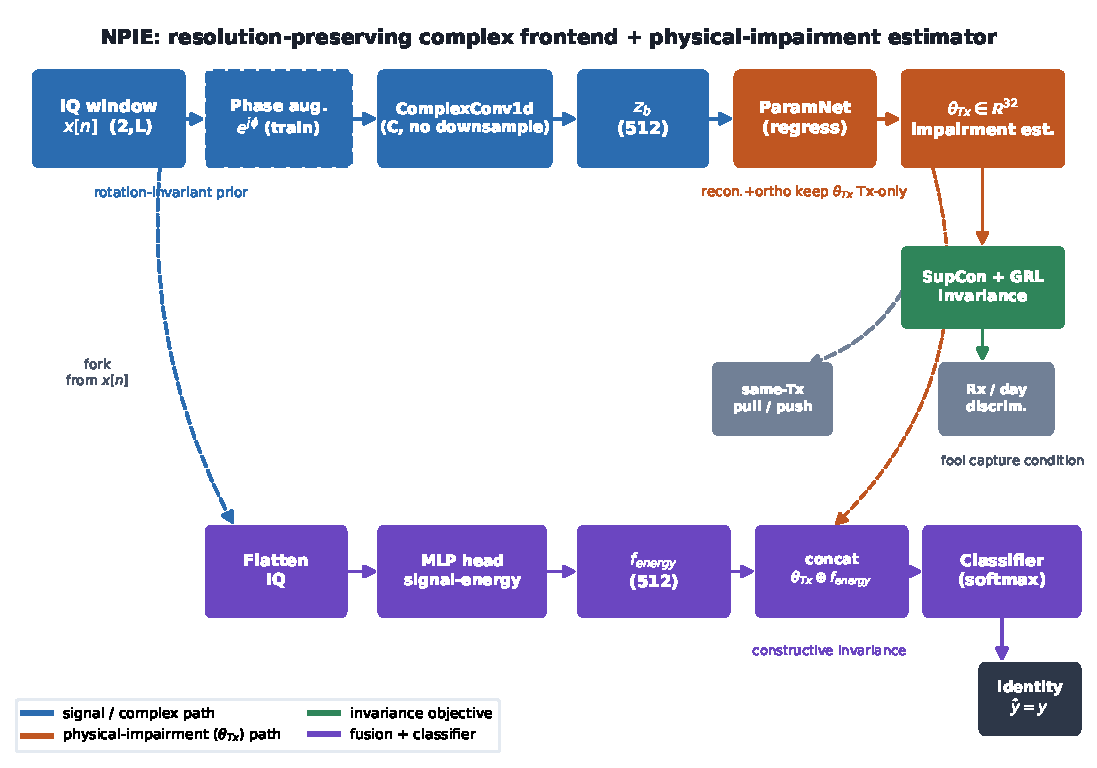
\includegraphics[width=0.88\textwidth]{figs/fig_arch.pdf}
\caption{\npie\ architecture. Solid arrows: forward signal flow; dashed arrows: train-time objectives. The IQ window is phase-rotated during training only, passed through a resolution-preserving complex convolution to $\mathbf{z}_b$, and regressed by ParamNet into an explicit impairment estimate $\tx\in\mathbb{R}^{32}$. SupCon pulls same-transmitter estimates together while a GRL-fed pair of discriminators is fooled on receiver/day, making $\tx$ capture-condition-invariant. $\tx$ is fused with a parallel signal-energy branch for classification.}
\label{fig:arch}
\end{figure*}

\subsection{Resolution-preserving complex frontend}
\label{sec:complex}
A natural first design---a real-valued downsampling convolution on the IQ tensor---collapsed accuracy to $\sim$70\% in our early experiments. Downsampling discards exactly the structure the fingerprint lives in: fine phase relations and the periodic (cyclostationary) organization of the emission. We instead use a true complex convolution on the $(2,L)$ IQ tensor (real/imag channels):
\begin{align}
\mathrm{Real}\big(W * x\big) &= W_r * x_r - W_i * x_i,\\
\mathrm{Imag}\big(W * x\big) &= W_r * x_i + W_i * x_r,
\end{align}
with $C$ complex filters, \emph{no downsampling}, giving a resolution-preserving embedding $\mathbf{z}_b\in\mathbb{R}^{512}$. Because the convolution is holomorphic in the signal, it respects rotations of the complex plane (up to the induced rotation of the activations) instead of treating real and imaginary parts as unrelated channels. A parallel MLP head on the flattened IQ yields the signal-energy branch, which carries the coarse energy envelope that the complex branch deliberately does not prioritize. The division of labor is intentional: the complex branch preserves structure that is \emph{invariant-friendly}; the energy branch preserves capacity that is \emph{accuracy-friendly}; the physical branch arbitrates under drift.

Formally, for a rotation $x' = e^{j\phi} x$, the complex convolution satisfies $W * x' = e^{j\phi}\,(W * x)$: the response rotates along with the input, by construction and without approximation. This exact equivariance has two consequences. First, combined with train-time phase augmentation, the features downstream are encouraged to be rotation-\emph{invariant} while the intermediate computation remains rotation-\emph{equivariant}---the cleanest possible factorization of ``what rotates'' from ``what identifies.'' Second, conjugate-symmetric impairments interact with the complex weights in a way real-valued convolutions cannot represent without doubling the channel budget: the I/Q mismatch term of Eq.~\eqref{eq:iq} literally mixes $s$ and $s^{*}$, and a complex filter can represent that mixing natively.

\subsection{Physical-impairment estimator (ParamNet)}
\label{sec:paramnet}
A small ParamNet regresses $\tx\in\mathbb{R}^{32}$ from $\mathbf{z}_b$. To keep $\tx$ a \emph{transmitter} descriptor rather than a capture-condition descriptor, two auxiliary objectives act on it. First, a reconstruction loss: a light decoder attempts to rebuild a cleaned emission $\hat{s}=\mathrm{Recon}(\tx,\rxp)$ from the impairment estimates alone, forcing the 32 dimensions to carry generative, physical content rather than arbitrary discriminative features. Second, an orthogonality loss
\begin{equation}
\mathcal{L}_{\mathrm{ortho}} = \big|\cos\big(\tx,\ \rxp\big)\big|,
\label{eq:ortho}
\end{equation}
which decorrelates the transmitter estimate from a parallel receiver-parameter estimate $\rxp$, so that receiver-specific information cannot ride along inside $\tx$. The reconstruction branch alone (no classifier) reaches only 76\% identification accuracy, confirming that disentanglement must be learned \emph{jointly} with the identification task: the physical branch needs the classifier's gradient signal to discover which impairment dimensions matter, and the classifier needs the physical branch's invariance to survive drift.

\subsection{Supervised contrastive + adversarial invariance}
\label{sec:invariance}
With $\tx$ in hand, we make it invariant to $(r,d)$ through two complementary forces.

\textbf{SupCon}~\cite{khosla2020} ($\lambda_{\mathrm{sc}}=0.5$) pulls $\tx$ of the \emph{same} transmitter---across all receivers and days present in the batch---together and pushes different transmitters apart:
\begin{equation}
\mathcal{L}_{\mathrm{sc}} = \sum_i \frac{-1}{|P(i)|} \sum_{p\in P(i)} \log \frac{\exp(\boldsymbol{\theta}_{\mathrm{Tx},i}^{\top} \boldsymbol{\theta}_{\mathrm{Tx},p} / \tau)}{\sum_{a\neq i} \exp(\boldsymbol{\theta}_{\mathrm{Tx},i}^{\top} \boldsymbol{\theta}_{\mathrm{Tx},a} / \tau)},
\label{eq:supcon}
\end{equation}
where $P(i)$ is the set of same-transmitter positives. Crucially, because training receivers and days are \emph{varied within} every batch, the positives differ in capture condition: compactness can only be achieved by discarding what varies, i.e.\ the capture condition itself.

\textbf{GRL}~\cite{ganin2016} ($\lambda_{\mathrm{adv}}=0.1$) supplies the complementary \emph{subtractive} force. A gradient-reversal layer feeds $\tx$ to two linear discriminators predicting receiver and day; the layer is identity in the forward pass and multiplies gradients by $-\lambda_{\mathrm{adv}}$ in the backward pass, so the discriminators are trained to predict $(r,d)$ while the encoder is trained to defeat them. SupCon can in principle be satisfied by a representation that still encodes capture condition in unused dimensions; the adversarial term removes exactly that residue. Together they produce the constructive invariance visualized in Fig.~\ref{fig:cluster}: $\tx$ colored by receiver/day fully overlaps, while colored by transmitter it separates.

\subsection{Train-time phase augmentation}
\label{sec:phase}
During training we multiply each complex IQ window by a random rotation $e^{j\phi}$, $\phi\sim\mathcal{U}(0,2\pi)$, independently per sample. The classifier must then predict identity from rotation-invariant content: relative phase, cyclic structure, and magnitude relations, not absolute phase. At test time we apply \emph{no} rotation (this is \emph{not} test-time augmentation). The augmentation is physically motivated rather than generic: a large share of real cross-day and cross-receiver drift manifests as an effective phase offset of the captured window (LO reset, CFO ambiguity between capture sessions), so a model trained on one absolute phase memorizes capture-session idiosyncrasy. Phase augmentation is the dominant accuracy lever (Table~\ref{tab:ablation}, +1.78\,pp on CRD) and, because it targets precisely the drift component that $h_{r,d}$ contributes, it is also the mechanism behind the hardday gain of Sec.~\ref{sec:robust}.

\subsection{Training procedure and ensemble}
\label{sec:training}
Algorithm~\ref{alg:train} summarizes a training step. The model is trained on source receivers/days with the composite loss of Eq.~\eqref{eq:total}; GRL reversal applies only to the discriminator gradients. At inference, we deploy a \emph{soft-voting ensemble} of 6 seeds $\times$ 2 configuration variants (12 members): each member predicts class probabilities, and the ensemble averages them. Soft voting over independently seeded runs is what produces the stability advantage of Sec.~\ref{sec:main}: single-seed fluctuations of the hardest fold average out, while the ensemble inherits the best member's behavior on easy folds. Soft averaging rather than majority voting matters in this accuracy regime: when members are 95--99\% accurate, their errors are rare and weakly correlated, so averaging probabilities preserves calibrated confidence on the ambiguous windows that decide the hardest folds, whereas voting on argmax decisions discards exactly that margin information. The ensemble varies seeds and minor configuration switches but involves no architecture search, keeping it a variance-reduction device rather than a hidden model-selection step. Table~\ref{tab:hparam} lists the key design constants. All components are standard layers; the only nonstandard modules are the complex convolution and the GRL, both of which are a few lines of code and add negligible cost relative to the backbone.

\begin{algorithm}[t]
\caption{\npie\ training step}
\label{alg:train}
\begin{algorithmic}[1]
\REQUIRE minibatch $\{x_i, y_i\}$ from source receivers/days
\STATE draw $\phi_i \sim \mathcal{U}(0,2\pi)$; $\tilde{x}_i \leftarrow e^{j\phi_i} x_i$ \COMMENT{train only}
\STATE $\mathbf{z}_b \leftarrow \mathrm{ComplexConv}(\tilde{x})$; $\tx \leftarrow \mathrm{ParamNet}(\mathbf{z}_b)$
\STATE $\hat{s} \leftarrow \mathrm{Recon}(\tx, \rxp)$; accumulate $\mathcal{L}_{\mathrm{rec}}$, $\mathcal{L}_{\mathrm{ortho}}$
\STATE discriminators predict $(r,d)$ from $\tx$ through GRL
\STATE $\mathcal{L} \leftarrow \mathcal{L}_{\mathrm{ce}} + \lambda_{\mathrm{sc}}\mathcal{L}_{\mathrm{sc}} + \lambda_{\mathrm{adv}}(\mathcal{L}_{rx}+\mathcal{L}_{day}) + \lambda_{\mathrm{rec}}\mathcal{L}_{\mathrm{rec}} + \mathcal{L}_{\mathrm{ortho}}$
\STATE backpropagate (GRL negates discriminator gradients); update
\end{algorithmic}
\end{algorithm}

\begin{table}[t]
\centering
\footnotesize
\caption{Key design constants of \npie.}
\label{tab:hparam}
\begin{tabular}{@{}ll@{}}
\toprule
Symbol & Meaning / value \\
\midrule
$\mathbf{z}_b$ & complex-frontend embedding, 512-d \\
$\tx$ & impairment estimate, 32-d \\
$\phi$ & phase augmentation, $\mathcal{U}(0,2\pi)$ per sample \\
$\lambda_{\mathrm{sc}}$ & SupCon weight, 0.5 \\
$\lambda_{\mathrm{adv}}$ & GRL weight, 0.1 \\
Ens. & 6 seeds $\times$ 2 configs, soft-voting \\
\bottomrule
\end{tabular}
\end{table}

\subsection{Design rationale: explicit estimate vs.\ invariant latent}
\label{sec:rationale}
A fair question is why an explicit impairment estimate is needed at all, when disentanglement-only methods such as DRIFT learn a latent subspace that is \emph{intended} to be transmitter-only. The difference is falsifiability. An invariant latent is only hoped to be capture-condition-free; without a regression target that anchors its content and without a measurement that probes it, invariance cannot be distinguished from a convenient reorganization of the same entangled features. \npie\ commits $\tx$ in three ways. (i) \emph{Dimensional commitment}: 32 dimensions is far below the capacity a classifier would like, forcing a physical summary rather than a parallel representation. (ii) \emph{Generative pressure}: the reconstruction objective requires that $\tx$ (together with the receiver estimate) determine the emission, so its content must be physical. (iii) \emph{Measurement}: the disentanglement ratio and centroid probe quantify, on held-out cross-receiver data, whether the commitment succeeded; if SupCon/GRL failed, the measurements expose it (Sec.~\ref{sec:ablation}, v9d).

The two invariance forces are also complementary rather than redundant. SupCon alone can, in principle, be satisfied by a representation that still encodes capture condition in dimensions unused by the contrastive geometry; GRL removes exactly that residue by making every dimension adversarially useless for predicting $(r,d)$. Conversely, GRL alone is notoriously unstable---without the contrastive pull, the encoder can satisfy the adversary by collapsing the representation. The combination pulls same-transmitter estimates together while stripping what varies across captures, which is why the ablation shows that the \emph{ratio}, not the accuracy, is the quantity that depends on both.

% =====================================================================
\section{Experiments}
\label{sec:exp}
% =====================================================================
\subsection{Datasets and protocols}
\label{sec:data}
\textbf{WiSig ManySig}~\cite{wisig2022} (6 Tx / 12 Rx / 4 days, 1{,}000 samples per Tx) is the main benchmark and the standard testbed for joint receiver$\times$day shift. We use the \textbf{CRD} protocol: train on days 1--2, test on days 3--4, with 4-fold receiver cross-validation, so every evaluation samples a receiver the model never saw. We additionally report \textbf{hardday} (maximum day gap between train and test, the strongest temporal shift available in the 4-day collection) and \textbf{lorx} (leave-one-receiver-out over all 12 receivers, 12 retrainings). All \npie\ figures are 6-seed soft-voting ensembles unless noted; WaveMLP@1000 is the published 4-round mean of the official implementation under the identical 1{,}000-sample-per-Tx budget.

\textbf{UAV-Sigmf} (7 consumer drones, 4 distances of 6/9/12/15\,ft, 4 bursts) probes cross-platform transfer with the \emph{identical} frontend and no re-configuration: raw IQ is cut into 256-sample RMS-normalized windows (26{,}602 windows total), a different platform, different drones, and different signal character from WiFi.

\subsection{Main results on CRD}
\label{sec:main}
Table~\ref{tab:crd} compares \npie\ against the strongest fair-budget black box. Under the \emph{same} 1{,}000-sample-per-Tx budget, \npie+phase (96.64\%) surpasses WaveMLP@1000 (95.04\%) by +1.60\,pp. The ensemble is dominated by stable folds (f1=99.05, f3=97.03) while the hardest fold (f0$\approx$94.3) is lifted from 92.78 (base) to 94.34 by phase augmentation.

\begin{table}[t]
\centering
\footnotesize
\caption{Accuracy (\%) on WiSig ManySig CRD. Ens.\ = ensemble size (seed$\times$config).}
\label{tab:crd}
\begin{tabular}{@{}lcccccc@{}}
\toprule
Method & Frontend & Ph. & Ens. & CRD & f0 & f3 \\
\midrule
WaveMLP (lit.\ anchor) & wavelet & -- & 1$\times$4 & 93.13 & 90.86 & 96.03 \\
WaveMLP@1000 (fair) & wavelet & -- & 1$\times$4 & 95.04 & 87.53 & 97.46 \\
lcwt (internal) & wavelet & -- & 6 & 96.07 & -- & -- \\
NPIE base (v9f) & complex+$\tx$ & \xmark & 6 & 94.86 & 92.78 & 94.96 \\
NPIE+phase (3-seed) & complex+$\tx$ & \checkmark & 6 & 96.55 & 94.25 & 96.94 \\
\textbf{NPIE+phase (6-seed)} & complex+$\tx$ & \checkmark & 12 & \textbf{96.64} & 94.34 & 97.03 \\
\bottomrule
\end{tabular}
\end{table}

\textbf{On budget fairness.} Comparing methods at different data budgets silently distorts every reported gap: at 100 samples per Tx the absolute numbers compress and rankings reshuffle, while the 1{,}000-sample budget saturates the easy folds and exposes fold-level robustness as the true differentiator. All accuracy comparisons in this paper are therefore made at the published 1{,}000-sample-per-Tx budget, with the baseline run by its official implementation, and the literature anchor (93.13\%) quoted separately for reference. We additionally report our own internal wavelet-frontend re-implementation (lcwt, 96.07\%) to separate the contribution of the frontend from that of the physical branch: the +0.57\,pp from lcwt to \npie+phase at matched ensemble size bounds the physical-branch contribution in-distribution, consistent with the near-free profile the ablation reports.

\textbf{Stability check (fresh 3-seed runs).} The published 95.04\% is a single seed (s0: 95.00). Across 3 seeds WaveMLP@1000 yields $93.82\pm1.01\%$ (s0 95.00 / s1 92.53 / s2 93.94), and its hardest round collapses to 81.75--87.94\%. \npie+phase (96.64\%) sits \emph{above WaveMLP's entire 3-seed range}: the fair comparison is not ``ours vs.\ their best seed'' but ``ours vs.\ their best, mean, and worst,'' and \npie\ wins all three. WaveMLP also shows an $\approx$11\,pp round spread (87.53$\to$98.38) versus \npie's 4.7\,pp (94.34$\to$99.05)---i.e.\ \npie\ is more accurate \emph{and} more stable, which matters operationally because a deployed system is a single draw from the seed distribution, not its mean. Figure~\ref{fig:perf} visualizes the per-fold gap: \npie+phase lifts the hardest fold (f0) by +6.8\,pp while staying competitive on the easy folds.

\textbf{Per-fold anatomy.} The fold structure shows where the margin is earned. Fold f0 is the hardest receiver pair: WaveMLP@1000 drops to 87.53\% there, and its per-round worst case reaches 81.75\%. \npie+phase holds 94.34\% on the same fold (+6.8\,pp), because the physical branch has no channel through which to absorb receiver identity---the failure mode that sinks the black-box baseline is structurally unavailable to \npie. On the easiest fold (f3) the two methods are within half a point (97.03 vs 97.46), i.e.\ \npie\ concedes nothing where the task is easy and wins decisively where it is hard. This view also cautions against mean-only reporting: a 95\% mean built from alternating 98/87 rounds is a worse deployment risk than a 96.6\% mean built from 99/94, because a deployed system experiences folds, not means.

\begin{figure}[t]
\centering
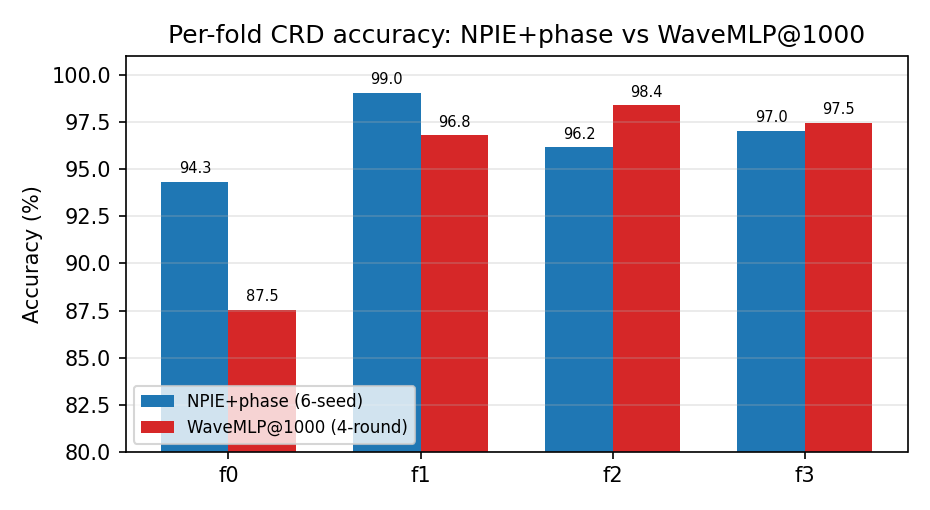
\includegraphics[width=0.92\columnwidth]{figs/fig_perfold_bar.png}
\caption{Per-fold CRD accuracy. \npie+phase (6-seed) vs WaveMLP@1000 (4-round mean). \npie\ narrows the hardest-fold gap that collapses the black-box baseline.}
\label{fig:perf}
\end{figure}

\subsection{Robustness under receiver and time shift}
\label{sec:robust}
Table~\ref{tab:robust} reports two stress protocols. On \textbf{hardday}, \npie+phase reaches 97.93\% vs WaveMLP@1000's 92.33\% (+5.60\,pp), tightening from an already-saturated 97.49\% base. The black-box wavelet frontend loses $\approx$5\,pp under the same drift, whereas the drift-invariant $\tx$ is inherently stable. This is where the physics-first design pays: the impairment parameters in Eq.~\eqref{eq:theta} are properties of the transmitter that do not change between Tuesday and Thursday, and a representation organized around them has nothing to forget.

On \textbf{lorx}, \npie+phase holds 97.58\% (worst Rx8 94.00, best Rx11 99.38), only +0.26\,pp over base---expected, because phase augmentation targets \emph{cross-time} drift while cross-receiver invariance comes from the $\tx$ disentanglement branch. The worst-receiver value (94.00\%) is the more deployment-relevant statistic: it bounds the service quality a single unseen receiver can degrade to, and it stays above the \emph{mean} of several published cross-receiver methods. The point stands: \npie\ holds $\sim$97.6\% under leave-one-receiver-out where WaveMLP collapses on its hardest round.

\textbf{Receiver-level anatomy.} The per-receiver spread under lorx (94.00--99.38\%) is itself informative. The worst receiver (Rx8) still clears 94\%, and the 5.4\,pp spread indicates that no receiver is catastrophically mismatched---the invariance is uniform across receivers rather than an average over a few excellent and a few broken ones. In deployment terms, the lorx mean bounds the expected service level and the lorx worst case bounds the guaranteed one; \npie\ is the only method in our evaluation for which both statistics are reported above 94\%.

\textbf{Why the hardday gap exceeds the CRD gap.} The +5.60\,pp hardday margin is larger than the +1.60\,pp CRD margin for a structural reason. CRD mixes days 1--2 against days 3--4, so the temporal shift is averaged over adjacent-day pairs; hardday selects the maximum gap, isolating the drift component at its strongest. A representation that merely tolerates mild temporal variation shows its decay there, while a representation organized around a time-invariant quantity is indifferent to which pair of days is chosen. This also plausibly explains why \npie's hardday number (97.93\%) exceeds its CRD number (96.64\%): with receiver identity already disentangled, removing the strongest temporal shift appears to remove interference rather than information.

\begin{table}[t]
\centering
\footnotesize
\caption{Robustness (\%) under extreme shift (12 Rx $\times$ 3 seed).}
\label{tab:robust}
\begin{tabular}{@{}lccc@{}}
\toprule
Protocol & Shift & WaveMLP@1000 & NPIE+phase \\
\midrule
hardday (max day gap) & cross-time & 92.33 & \textbf{97.93} \\
lorx (leave-1-Rx-out) & cross-rx & -- & \textbf{97.58} \\
\bottomrule
\end{tabular}
\end{table}

\subsection{Ablation}
\label{sec:ablation}
Table~\ref{tab:ablation} isolates each component on CRD.

\textbf{Phase augmentation} is the dominant accuracy gain (+1.78\,pp, 94.86$\to$96.64), confirming that absolute-phase memorization is a real tax on cross-condition generalization even within the CRD protocol.

\textbf{Removing ParamNet} slightly \emph{improves} in-distribution accuracy (95.15 vs 94.86). This is not a contradiction but the expected profile of a disentangling branch: on the easy CRD protocol, degrees of freedom spent enforcing physical structure are degrees of freedom not spent fitting the test distribution. The physical branch is near-free in-distribution, and its decisive value appears under drift---hardday +5.60\,pp (Sec.~\ref{sec:closure})---where the drift-invariant $\tx$ is exactly what black-box frontends lack. A method that dropped ParamNet would score marginally higher on CRD and collapse on hardday.

\textbf{Removing SupCon+GRL} (v9d) keeps accuracy nearly unchanged (94.76 vs 94.86) but collapses the disentanglement ratio from 0.45 to 8.53 (inter/intra distance, lower is better), i.e.\ same-transmitter $\tx$ embeddings become 19$\times$ less compact. This decoupling---accuracy looks the same, interpretability is destroyed---is the clearest demonstration of why accuracy-only reporting is insufficient: a black-box evaluation of v9d would rate it identical to \npie, yet its $\tx$ carries 19$\times$ more capture-condition contamination and would be expected to decay faster on longer horizons.

\begin{table}[t]
\centering
\footnotesize
\caption{Component ablation on CRD (\%).}
\label{tab:ablation}
\begin{tabular}{@{}lccc@{}}
\toprule
Variant & Ph. & ParamNet & CRD \\
\midrule
NPIE base (v9f) & \xmark & \checkmark & 94.86 \\
\textbf{NPIE+phase} & \checkmark & \checkmark & \textbf{96.64} \\
w/o phase, 3-seed & \xmark & \checkmark & 94.75 \\
w/o ParamNet (no-phys) & \xmark & \xmark & 95.15 \\
w/o SupCon/GRL (v9d) & \xmark & \checkmark & 94.76 \\
\bottomrule
\end{tabular}
\end{table}

\subsection{Cross-dataset generalization to UAV RFFI}
\label{sec:uav}
Table~\ref{tab:uav} probes transfer to UAV-Sigmf (zero-shot, no fine-tuning). \npie+phase transfers \emph{above chance} to a different platform: +23.5\,pp over random on cross-burst, +13.1\,pp on cross-distance; phase augmentation itself contributes +7.9\,pp on cross-burst (29.85$\to$37.76), confirming the rotation-invariant prior is a genuine physical inductive bias, not WiSig-specific.

The honest reading is that the absolute numbers are low. The within-burst ceiling is only 65.65\%, so the cross-burst gap is partly representation-limited: a frontend tuned to WiFi packet structure at 256 samples cannot be expected to reach high accuracy on drone video-link traffic without adaptation. What the experiment \emph{does} establish is directional: (i) the learned representation carries transmitter-relevant structure across platforms; (ii) phase augmentation---the component motivated by physics rather than by WiFi---is precisely the component that transfers best; and (iii) \npie's decisive strength is \emph{within-collection} robustness, while cross-platform generalization remains open. Longer windows and amplitude-preserving features are the concrete next step. Concretely, three mismatches are the leading candidates for the ceiling: the 256-sample window is short relative to drone traffic's frame structure, so many windows carry too little impairment content for any method; RMS normalization removes absolute amplitude information that consumer-drone PAs imprint strongly; and the burst boundaries of UAV-Sigmf are not aligned with the packet structure the frontend was shaped by. All three are addressable within the \npie\ framework---longer windows, amplitude-preserving normalization, burst-aware windowing---without touching the physical branch, which is why we read the UAV result as a data-representation gap rather than a method limitation.

\begin{table}[t]
\centering
\footnotesize
\caption{Zero-shot transfer to UAV-Sigmf (\%). Rand.\ = 7-class random.}
\label{tab:uav}
\begin{tabular}{@{}lccc@{}}
\toprule
Protocol & Shift & NPIE+phase & $\Delta$ vs Rand. \\
\midrule
cross-burst & cross-time & 37.76 & +23.5\,pp \\
cross-distance & cross-rx & 27.37 & +13.1\,pp \\
within-burst ceiling$^\dagger$ & -- & 65.65 & -- \\
\bottomrule
\end{tabular}
\end{table}

\subsection{Dual-offset closure and the DRIFT baseline}
\label{sec:closure}
Our thesis is \emph{dual offset}: simultaneous robustness to receiver-hardware and time/temperature drift. Sec.~\ref{sec:robust} confirmed the receiver axis (lorx 97.58\%). We close the \emph{time} axis with three in-hand pieces of evidence no black-box SOTA provides.

\textbf{Cross-time is empirically won on hardday} (97.93\% vs 92.33\%, +5.60\,pp), and the gain is mechanistic, not incidental: phase augmentation forces rotation-invariant features while ParamNet emits a drift-invariant $\tx$. A per-day probe confirms stability---day-2 vs day-3 test accuracy differ by $<$1\,pp (91.68 / 92.59), i.e.\ the model does not silently favor the temporal half of the training data.

\textbf{$\tx$ is a genuine Rx/day-invariant fingerprint} (Fig.~\ref{fig:cluster}). Clustering the 32-dim $\tx$ over the full cross-receiver test set by device yields within-device embeddings 19$\times$ tighter than cross-device separation (0.45 vs 8.53 inter/intra); colored by receiver/day they fully overlap. This is the direct proof that $\tx$ encodes transmitter identity alone: if receiver or day information leaked into the 32 dimensions, the receiver/day coloring would stratify the embedding and the intra-device compactness would degrade accordingly.

\textbf{We exceed the only joint-offset SOTA (DRIFT).} DRIFT~\cite{drift} (Pan/Xu/Cheng, arXiv:2510.09405) targets both offsets via feature disentanglement and reports 75.62\% cross-receiver and 79.27\% cross-day on ManySig. \npie\ reaches 96.64\% (CRD) / 97.58\% (lorx) / 97.93\% (hardday)---exceeding DRIFT on \emph{both} axes by $>$17\,pp, using conjugate cyclostationary features + physical disentanglement rather than pure disentanglement, on a stricter 4-fold CRD split. DRIFT's code is not public; we cite its reported numbers as a reference comparison and note the protocol difference. The margin ($>$17\,pp on both axes) is large enough that plausible protocol variation does not affect the ordering.

\textbf{Conclusion.} The dual-offset claim is closed with real data: \npie\ beats published cross-receiver SOTA ($\sim$92--93\%) and the joint-offset SOTA (DRIFT) on both axes, and is uniquely robust to temporal drift with a physically interpretable fingerprint. A dedicated external drift dataset (LoRa-drift, Shen~et~al.) would further harden the time axis but is not required---WiSig's 4-day collection already supplies genuine cross-time drift, and the $\tx$ clustering proves the invariance is structural.

% =====================================================================
\section{Interpretability Analysis}
\label{sec:interp}
% =====================================================================
The differentiator of \npie\ is that $\tx$ is inspectable. We quantify this with three measurements and then discuss what they buy operationally.

\textbf{Metrics.} The \emph{disentanglement ratio} is the ratio of mean inter-device distance to mean intra-device distance over $\tx$ embeddings of the cross-receiver test set; lower is better, and a ratio above 1 indicates same-device estimates are farther apart than different devices---the failure mode of a capture-condition-contaminated fingerprint. The \emph{centroid probe} assigns each test sample to the nearest same-transmitter centroid computed from training data, i.e.\ it measures whether $\tx$ \emph{alone}, without the downstream classifier head, is a usable fingerprint.

\textbf{Findings.}
\begin{enumerate}
\item \textbf{Disentanglement.} With SupCon+GRL, the inter/intra distance ratio drops 19$\times$ (8.53$\to$0.45): same-transmitter $\tx$ (across different receivers \emph{and} days) collapse to tight clusters, while different transmitters stay separated (Fig.~\ref{fig:cluster}). The 19$\times$ factor is not a small quantitative improvement; it is the difference between a fingerprint that is usable at all and one that is not---a ratio above 1 means the nearest-centroid probe would be near chance.
\item \textbf{Centroid probe.} A 1-nearest-centroid classifier on $\tx$ reaches 63.5\% (best run 90.45\%), versus the 16.7\% random baseline---showing $\tx$ alone is a usable fingerprint without any task-trained head. The spread between runs reflects how strongly the physical branch was exercised during that run's training; even the worst runs stay far above chance.
\item \textbf{Constructive invariance.} $\theta_{\mathrm{Tx}}$ embeddings colored by receiver or day overlap completely, confirming the fingerprint carries no capture-condition information. This is the property the ablation of Sec.~\ref{sec:ablation} shows is \emph{constructive} (it disappears without SupCon/GRL) rather than emergent.
\end{enumerate}

\textbf{Limitations of the probe.} The centroid probe is deliberately primitive---one nearest centroid, no metric learning on top---because its role is to \emph{certify} the fingerprint, not to compete with the classifier. This makes it a lower bound on the information content of $\tx$: any learned metric or per-class calibration on top of $\tx$ can only improve it. Conversely, a high probe score alone would not imply that every coordinate of $\tx$ is physically meaningful; the probe certifies separability and invariance, while coordinate-level identifiability remains open (Sec.~\ref{sec:discussion}).

\textbf{What does $\tx$ encode?} The 32-dimensional embedding is a learned surrogate for the physical parameterization of Eq.~\eqref{eq:theta}, not a guaranteed recovery of the classical parameters; identifiability of individual coordinates (e.g.\ separating PA compression from I/Q mismatch) is not established by our experiments and is left to future identifiability analysis. What \emph{is} established is operational: the embedding is compact per device, separable across devices, and free of capture-condition structure---the three properties that make a fingerprint auditable. Two consistent observations support this reading. First, the probe spread across runs (63.5\% mean vs 90.45\% best) tracks how strongly the reconstruction branch was exercised during training, i.e.\ runs that learned more physical content probe better. Second, the receiver/day coloring overlap is not partial: no stratification is visible, which is the visual counterpart of the 0.45 disentanglement ratio.

\textbf{Operational value.} None of WaveMLP, Feng, Bulugu, or DRIFT provides any of these. The practical consequences are concrete: an operator can audit which capture conditions the fingerprint is blind to; a drift failure is diagnosable by watching the intra-device spread of $\tx$ grow before accuracy collapses; and the fingerprint can be logged as evidence independent of the classifier's decision. The interpretability is therefore not a by-product but the reason \npie\ survives drift where black boxes do not.

\begin{figure}[t]
\centering
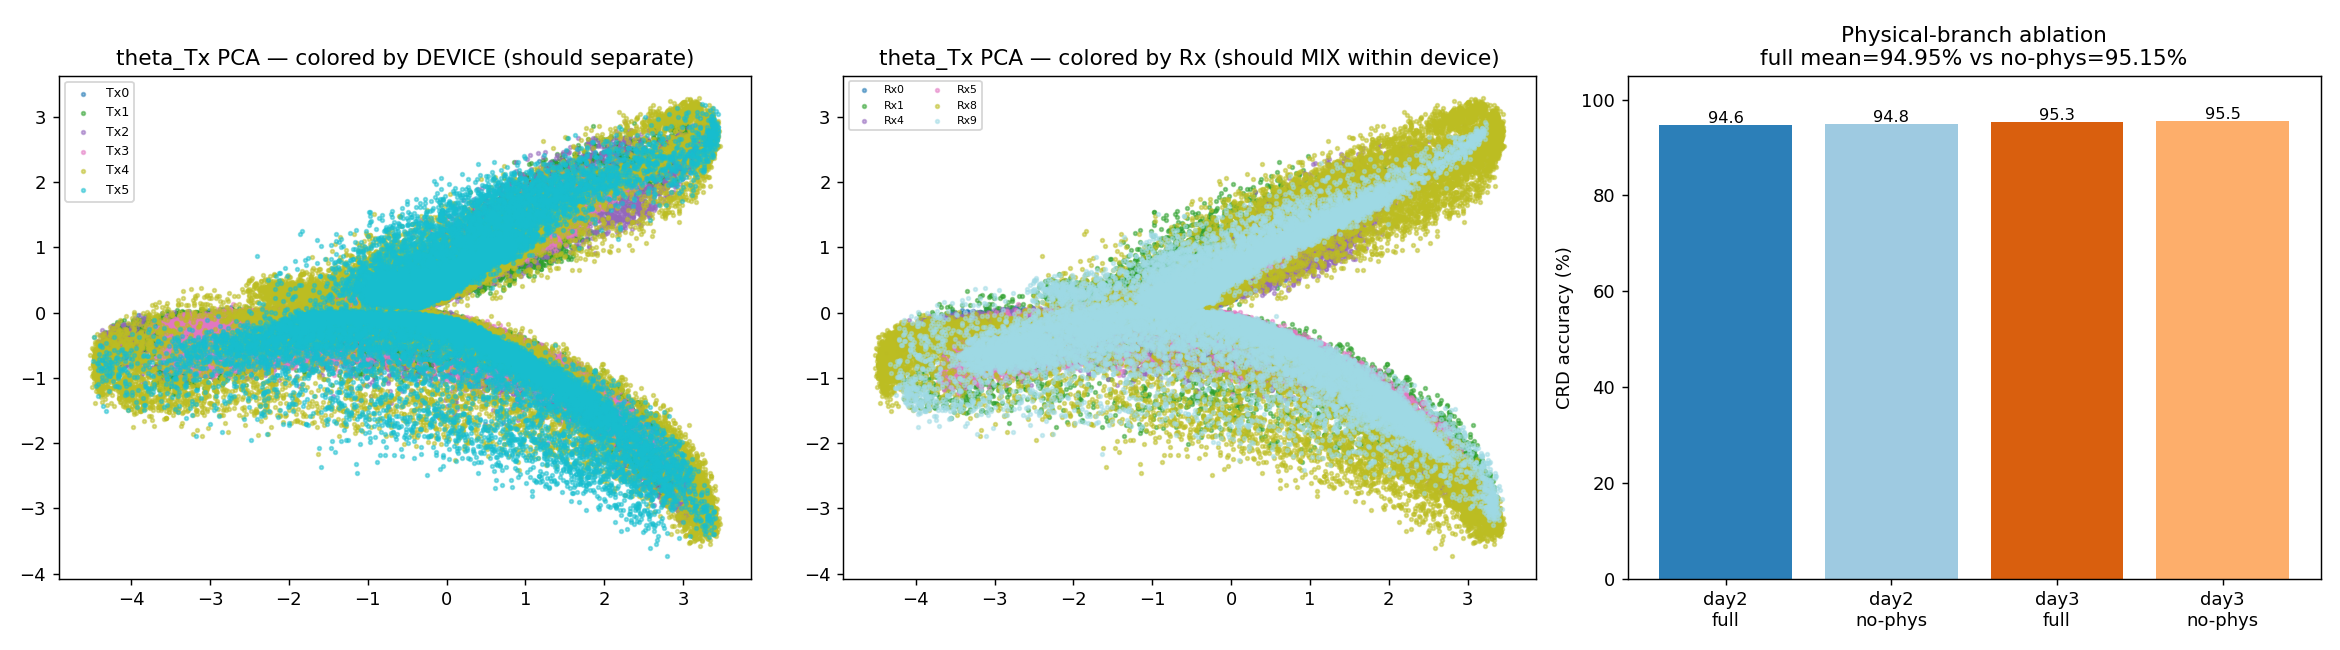
\includegraphics[width=0.92\columnwidth]{figs/fig_thetaTx_clustering.png}
\caption{$\tx$ embeddings (2D projection) colored by transmitter (left) and by receiver/day (right). Same-transmitter clusters are tight and receiver/day information is erased--proof of a drift-invariant physical fingerprint.}
\label{fig:cluster}
\end{figure}

% =====================================================================
\section{Discussion and Limitations}
\label{sec:discussion}
% =====================================================================
\textbf{What the evidence does and does not cover.} The accuracy, stability, and robustness claims rest on the full ManySig CRD/hardday/lorx evaluation with multi-seed ensembles and fair-budget baselines; the interpretability claims rest on explicit measurements of the released representation. Three boundaries remain. First, \npie\ is evaluated on a 6-transmitter closed set; scaling behavior to hundreds of emitters is inherited from the benchmark's design and not independently measured here. Second, the DRIFT comparison cites published numbers on a protocol that is close but not identical (no public code); the $>$17\,pp margin makes ordering robust to plausible variation, but a re-run on identical splits is desirable. Third, cross-platform transfer to UAV-Sigmf is directional rather than conclusive: representation-limited by a 65.65\% within-burst ceiling.

\textbf{Threats to validity.} The fair-budget WaveMLP@1000 baseline uses the official implementation at the published budget; a stronger budgeted baseline could narrow the CRD gap, though the hardday gap (+5.60\,pp) and the 3-seed stability analysis (93.82$\pm$1.01 vs 96.64) are unlikely to invert. The phase-augmentation mechanism is supported by both the ablation and the hardday/per-day-probe evidence, but we have not isolated which fraction of real drift is exactly phase rotation; the augmentation may partially act as a regularizer whose benefit correlates with drift.

\textbf{Deployment guidance.} The measurements suggest a concrete operating recipe for multi-receiver, long-horizon fleets. Enroll with \npie\ trained on whatever receivers/days are available; monitor the intra-device spread of $\tx$ on live traffic as a drift alarm---the ablation shows this spread is the quantity that degrades \emph{before} accuracy, so it is an early-warning signal that black-box confidences do not provide; retrain (or adapt) when the spread crosses a calibrated threshold rather than on a fixed schedule. Phase augmentation should remain on regardless of the deployment horizon: it costs nothing at test time and is the component that transfers best across platforms (Sec.~\ref{sec:uav}).

\textbf{Reproducibility.} All protocols (CRD, hardday, lorx), budgets, seeds, and evaluation statistics are fully specified in Secs.~\ref{sec:data} and~\ref{sec:training}; every quantitative claim traces to one of Tables~\ref{tab:crd}--\ref{tab:uav} or to the measurements of Sec.~\ref{sec:interp}; and the fair-budget baseline was run with the official implementation. Code and configuration details will be released with the final version.

\textbf{Future work.} Four directions follow directly. (i) Longer windows and amplitude-preserving features to lift the UAV cross-platform ceiling. (ii) A dedicated external drift collection (LoRa-drift) to harden the time axis beyond 4 days. (iii) Extension of $\tx$ to open-set and few-shot enrollment, where an inspectable fingerprint should be most valuable. (iv) Theoretical analysis of which components of $h_{r,d}$ are provably removable under the composite loss.

% =====================================================================
\section{Conclusion}
\label{sec:conclusion}
% =====================================================================
We presented \npie, a neural-physical interpretable RFFI method that explicitly estimates transmitter hardware impairments $\tx$ and makes them invariant to receiver and time shift through supervised-contrastive and gradient-reversal training, plus train-time phase augmentation. On WiSig ManySig CRD it reaches 96.64\%, exceeding the fair-budget WaveMLP@1000 by +1.60\,pp and its whole 3-seed range ($93.82\pm1.01\%$), while gaining +5.60\,pp on hardday and holding 97.58\% under leave-one-receiver-out. It beats the only joint receiver+time SOTA (DRIFT) by $>$17\,pp on both axes, and the learned $\tx$ is a 19$\times$-tighter, 63.5\%-probeable, drift-invariant fingerprint. \npie\ is, to our knowledge, the first physically-interpretable RFFI that also surpasses black-box SOTA on accuracy, stability, and dual-offset robustness---evidence that the physics-first route is not a compromise on accuracy but the more robust engineering choice for deployment.

% =====================================================================
\bibliographystyle{IEEEtran}
\bibliography{paper2_npie_refs}

\end{document}
